\subsection{Public Communication Crew}

The Public Communication Crew operates within a structured \textbf{sequential process} to ensure efficient and accurate communication of fire incident reports to the public. Each task is assigned to a specific agent with well-defined responsibilities, as detailed below:

\begin{enumerate}
	\item \textbf{Receive Report:} The \textit{Communication Operator} obtains the fire incident report in Markdown format. This serves as the starting point for the process and can filter any information that is not relevant for this crew.
	\item \textbf{Search Related Cases:} The \textit{Archive Keeper} searches for past incidents with similar locations or fire types. This task depends on the completion of the \textit{Receive Report} task.
	\item \textbf{Draft Initial Article:} The \textit{Article Writer} drafts an initial article based on the current report. This task also depends on the completion of the \textit{Receive Report} task.
	\item \textbf{Integrate Additional Information:} The \textit{Article Writer} integrates insights from related cases into the draft. This task requires the completion of both the \textit{Search Related Cases} and \textit{Draft Initial Article} tasks.
	\item \textbf{Review and Authorize Publication:} The \textit{Mayor} reviews the article and either authorizes publication or provides feedback for revisions. This task depends on the completion of the \textit{Integrate Additional Information} task.
	\item \textbf{Provide Social Media Feedback:} The \textit{Social Media Commentator} critiques the emergency response in a humorous yet constructive manner. This task depends on the approval of the article by the \textit{Mayor}.
\end{enumerate}

\begin{figure}[ht!]
	\centering
	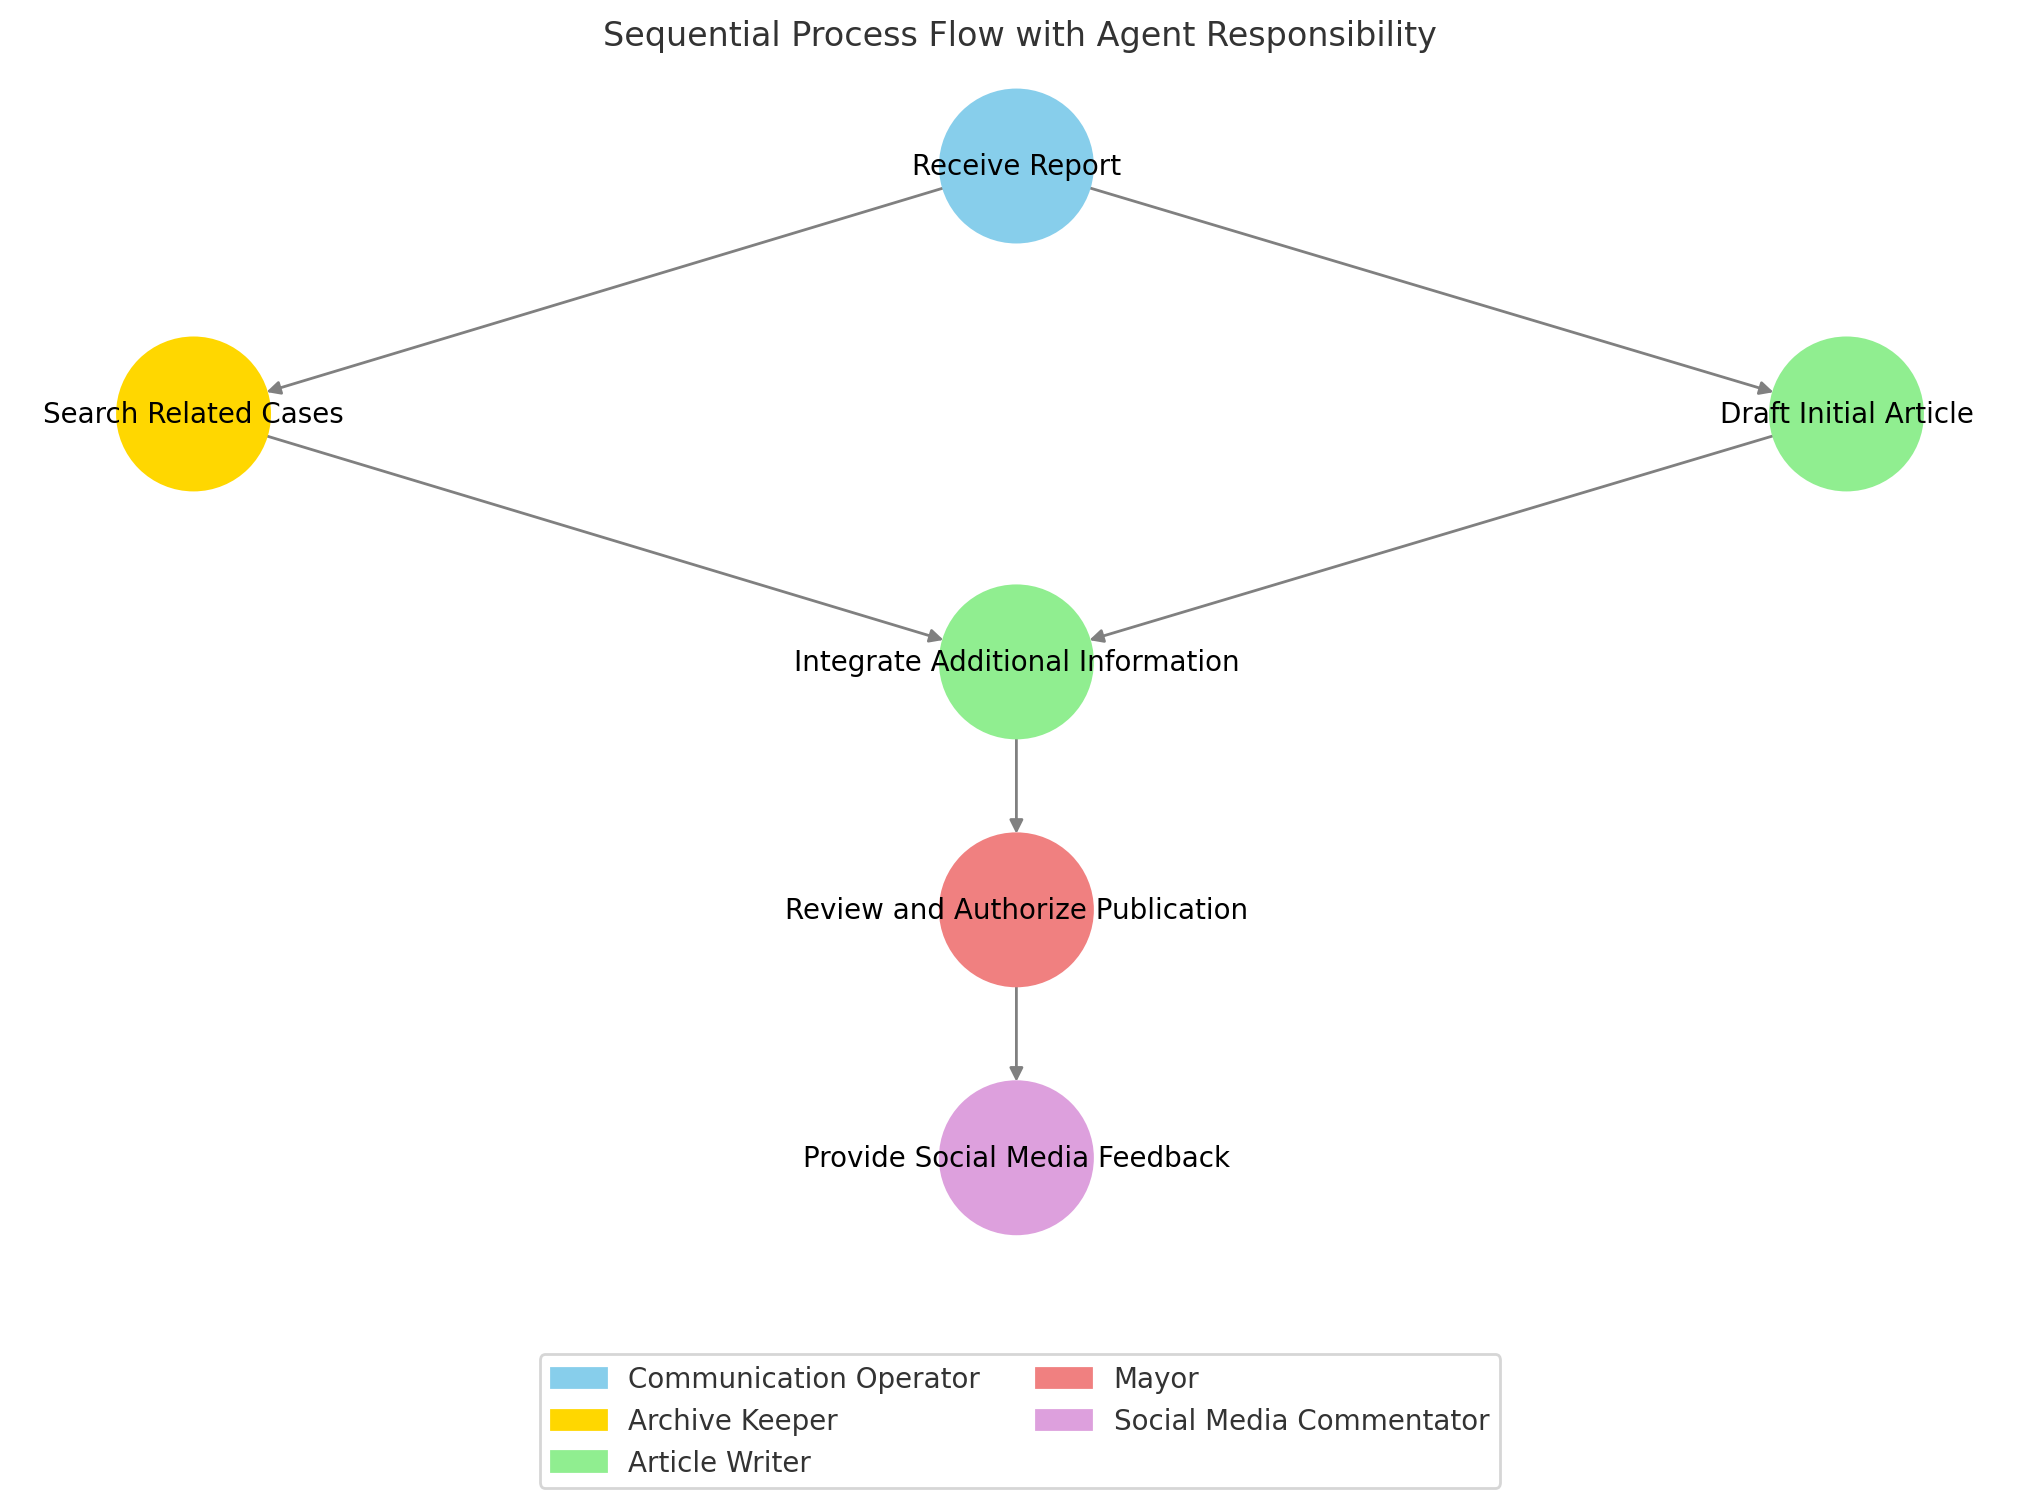
\includegraphics[width=0.9\textwidth]{figures/PC-process.png}
	\caption{Sequential Process Flow of the Public Communication Crew with Agent Responsibilities}
	\label{fig:public_comm_flow}
\end{figure}


\paragraph{Task Dependencies}
The sequential process relies on strict task dependencies to ensure an organized workflow:
\begin{itemize}
	\item \textit{Search Related Cases} and \textit{Draft Initial Article} can be executed in parallel but both depend on \textit{Receive Report}.
	\item \textit{Integrate Additional Information} requires the completion of both \textit{Search Related Cases} and \textit{Draft Initial Article}.
	\item \textit{Review and Authorize Publication} depends on \textit{Integrate Additional Information}.
	\item \textit{Provide Social Media Feedback} requires article approval from the \textit{Mayor}.
\end{itemize}

The visual representation in Figure~\ref{fig:public_comm_flow} highlights these dependencies and assigns colors to denote the responsible agents, ensuring clarity and accountability.
